\section{Comparison between data and prediction}
The requirement of at least two $b$-tagged jets selects a sample dominated by $t\bar{t}+$jets. Thus data-to-MC comparisons at preselection level give the possibility to validate the modelling of the main backgrounds. Figures \ref{sec:vlq:fig:1ldatamc} and \ref{sec:vlq:fig:0ldatamc} show basic kinematic variables at preselection level  in both 1-lepton and 0-lepton channels.
 

\begin{figure}[p]
\begin{subfigure}{0.33\textwidth}
  \centering
  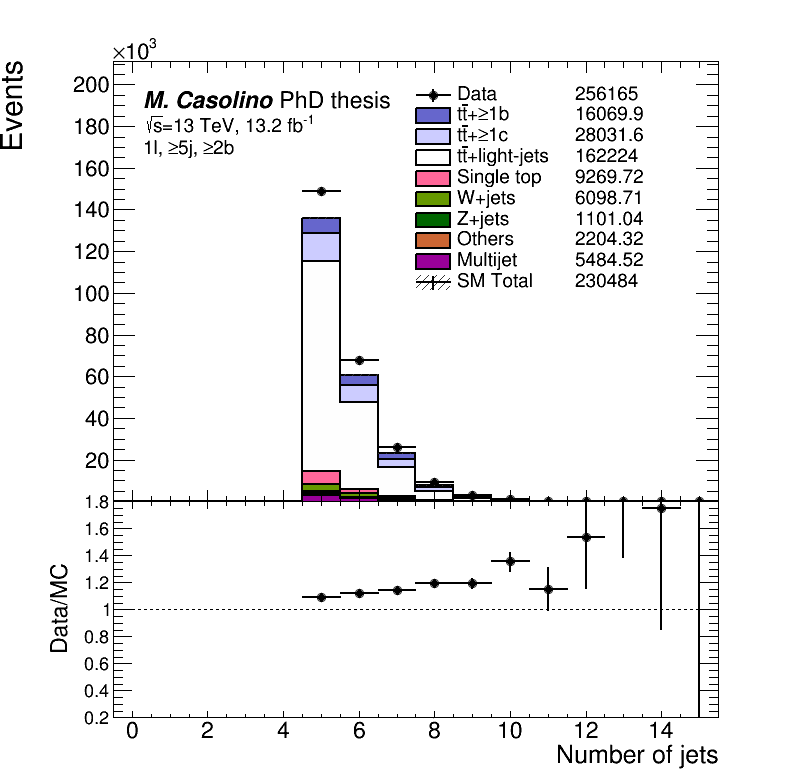
\includegraphics[width=0.9\textwidth]{figures/VLQ/presel/1lep/canv_c1l2b_jets_n.png}
  \caption{}
  \label{}
\end{subfigure}
\begin{subfigure}{0.33\textwidth}
  \centering
  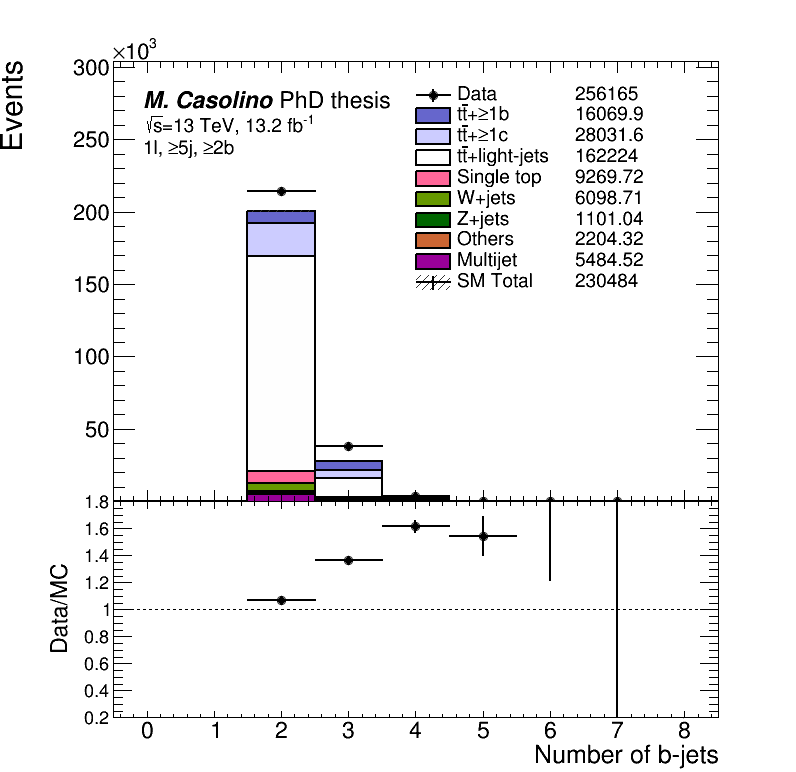
\includegraphics[width=0.9\textwidth]{figures/VLQ/presel/1lep/canv_c1l2b_bjets_n.png}
  \caption{}
  \label{}
\end{subfigure}
\begin{subfigure}{0.33\textwidth}
  \centering
  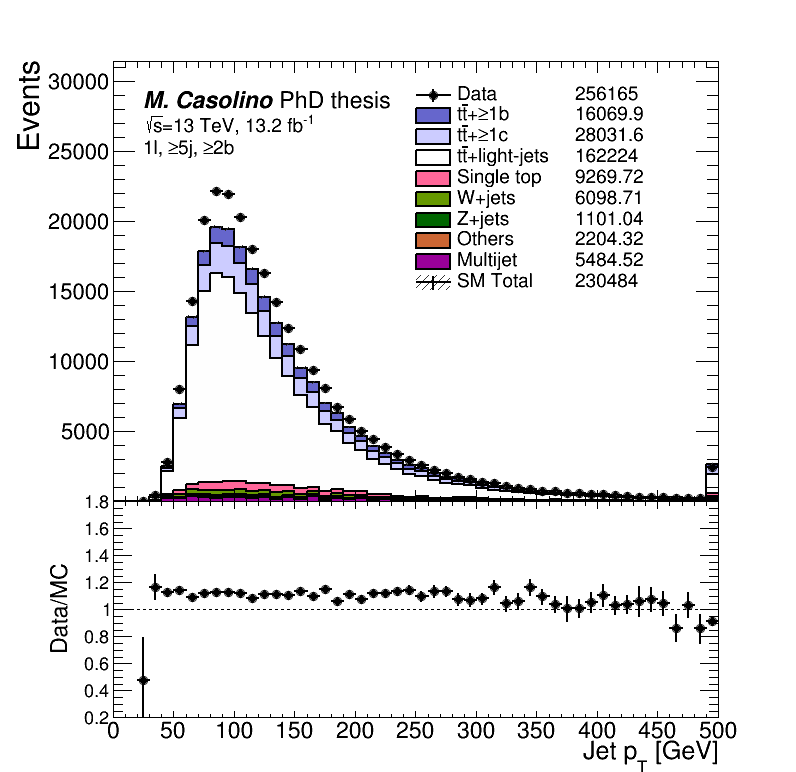
\includegraphics[width=0.9\textwidth]{figures/VLQ/presel/1lep/canv_c1l2b_jet0_pt.png}
  \caption{}
  \label{}
\end{subfigure}
\begin{subfigure}{0.33\textwidth}
  \centering
  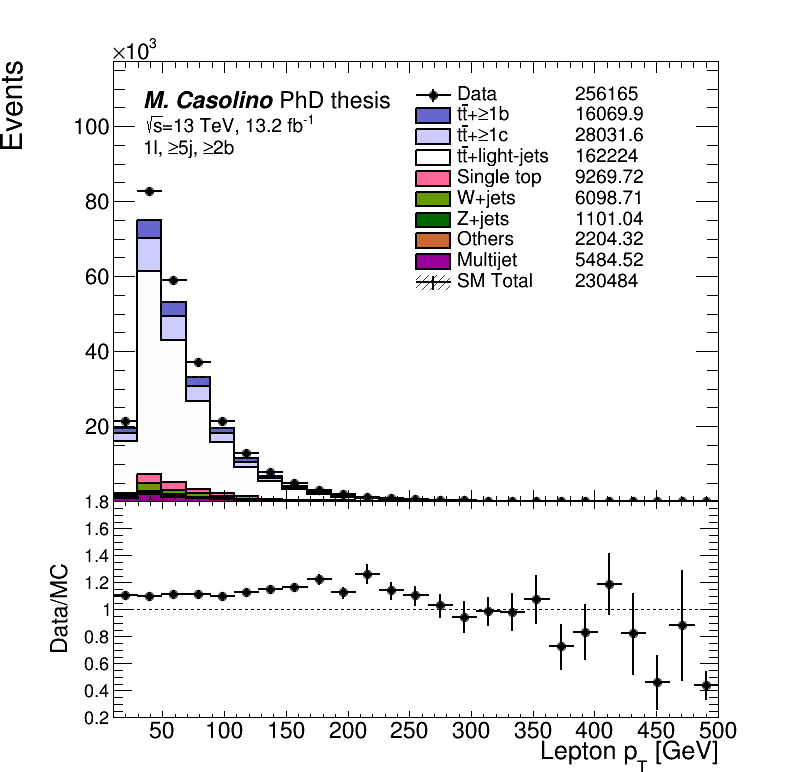
\includegraphics[width=0.9\textwidth]{figures/VLQ/presel/1lep/canv_c1l2b_lep0_pt_zoom.png}
  \caption{}
  \label{}
\end{subfigure}
\begin{subfigure}{0.33\textwidth}
  \centering
  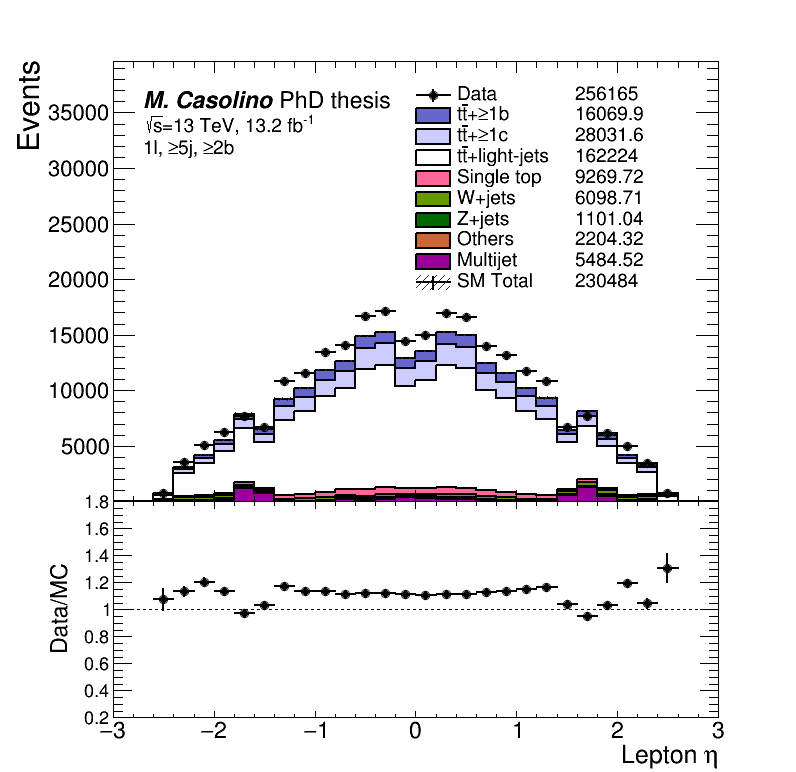
\includegraphics[width=0.9\textwidth]{figures/VLQ/presel/1lep/canv_c1l2b_lep0_eta.png}
  \caption{}
  \label{}
\end{subfigure}
\begin{subfigure}{0.33\textwidth}
  \centering
  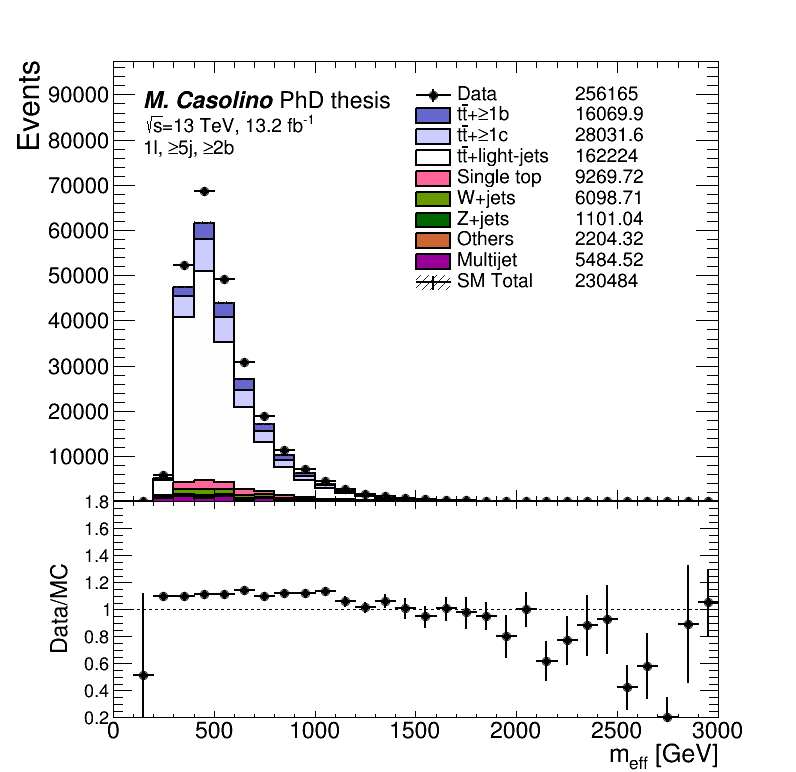
\includegraphics[width=0.9\textwidth]{figures/VLQ/presel/1lep/canv_c1l2b_meff.png}
  \caption{}
  \label{}
\end{subfigure}
\begin{subfigure}{0.33\textwidth}
  \centering
  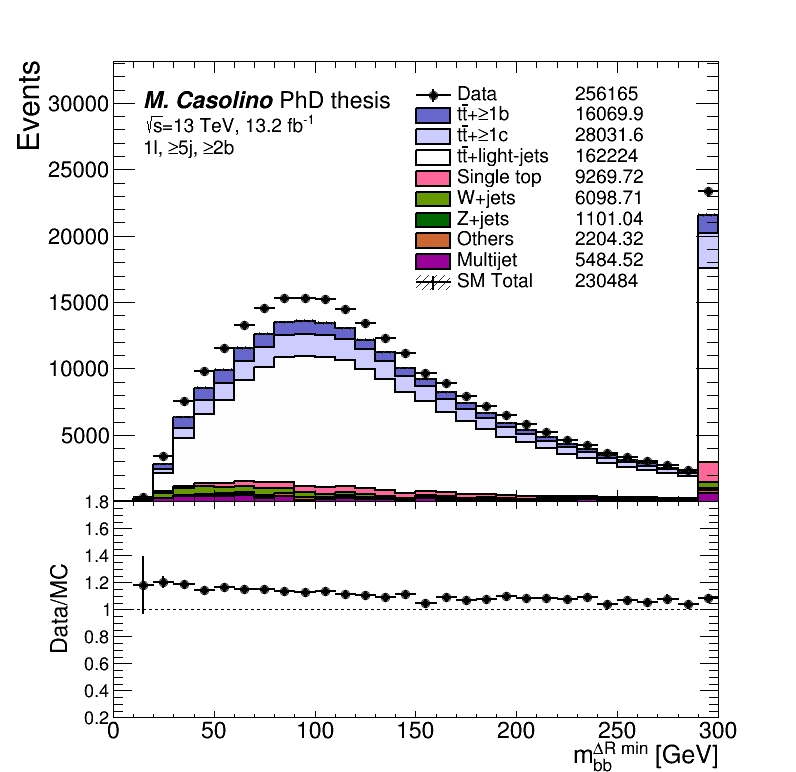
\includegraphics[width=0.9\textwidth]{figures/VLQ/presel/1lep/canv_c1l2b_mbb_mindR.png}
  \caption{}
  \label{}
\end{subfigure}
\begin{subfigure}{0.33\textwidth}
  \centering
  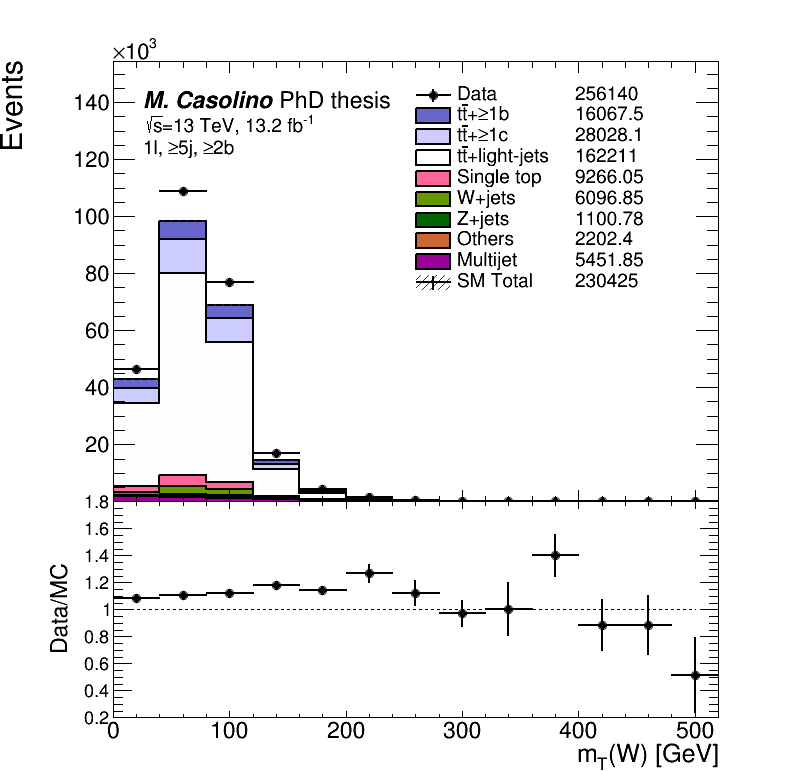
\includegraphics[width=0.9\textwidth]{figures/VLQ/presel/1lep/canv_c1l2b_mtw.png}
  \caption{}
  \label{}
\end{subfigure}
\begin{subfigure}{0.33\textwidth}
  \centering
  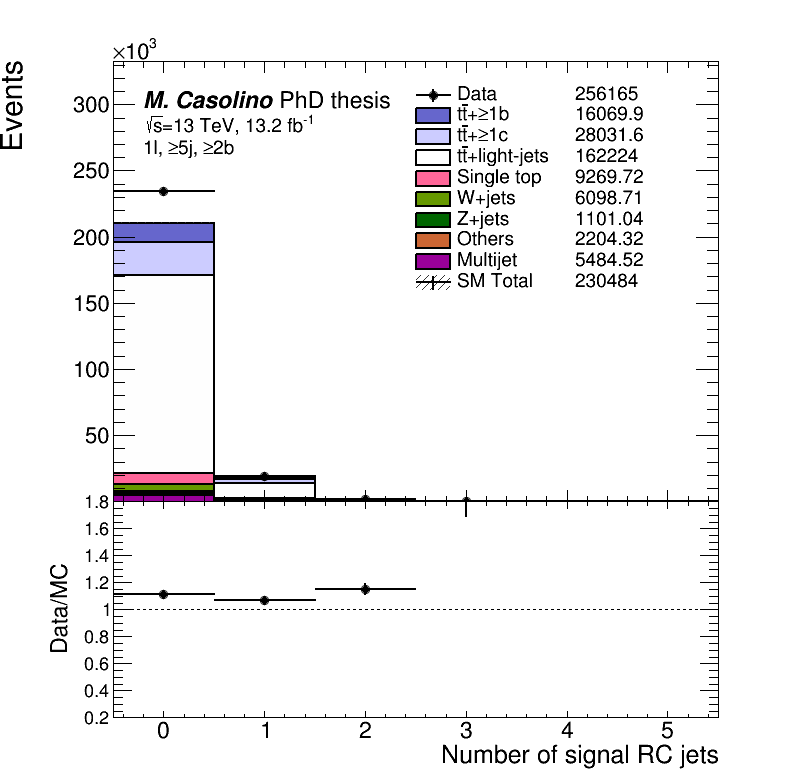
\includegraphics[width=0.9\textwidth]{figures/VLQ/presel/1lep/canv_c1l2b_RCjets_n.png}
  \caption{}
  \label{}
\end{subfigure}
\captionsetup{width=0.85\textwidth} \caption{\small Comparison between data and prediction in 1-lepton channel for (a) jet multiplicity, (b) $b$-tag multiplicity, (c) leading jet $\pt$, (d) lepton $\pt$, (e) lepton $\eta$, (f) $m_{\rm eff}$, (g) invariant mass of the closest $b$-jets pair ($m_{bb}^{{\rm min}\Delta R}$) , (h) transverse mass of the $W$ boson $m_{\rm T}^{W}$, and (j) RT-jet multiplicity.}
\label{sec:vlq:fig:1ldatamc}
\end{figure}



\begin{figure}[p]
\begin{subfigure}{0.33\textwidth}
  \centering
  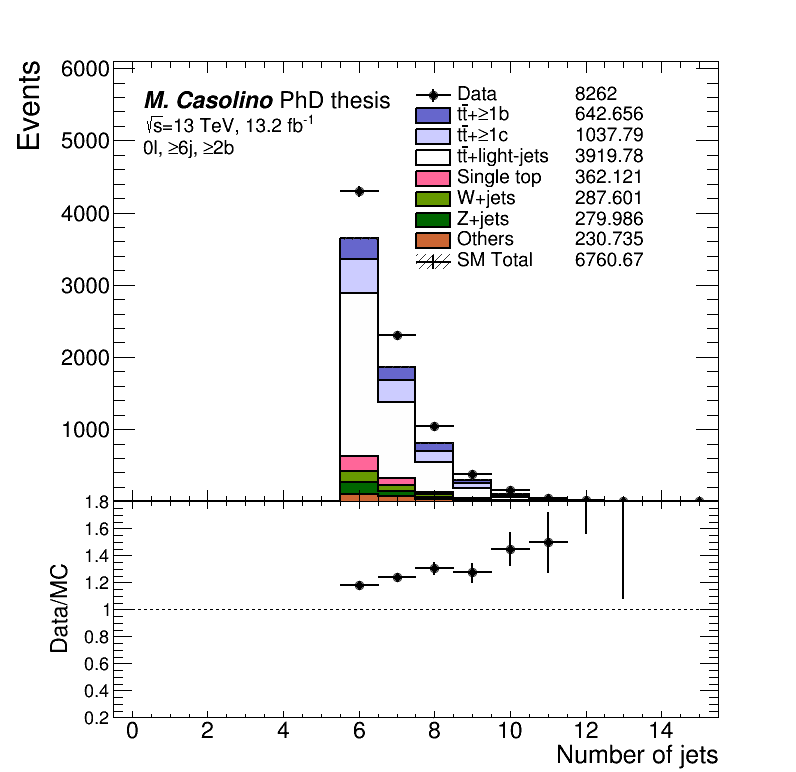
\includegraphics[width=0.9\textwidth]{figures/VLQ/presel/0lep/canv_c0l2b_jets_n.png}
  \caption{}
  \label{}
\end{subfigure}
\begin{subfigure}{0.33\textwidth}
  \centering
  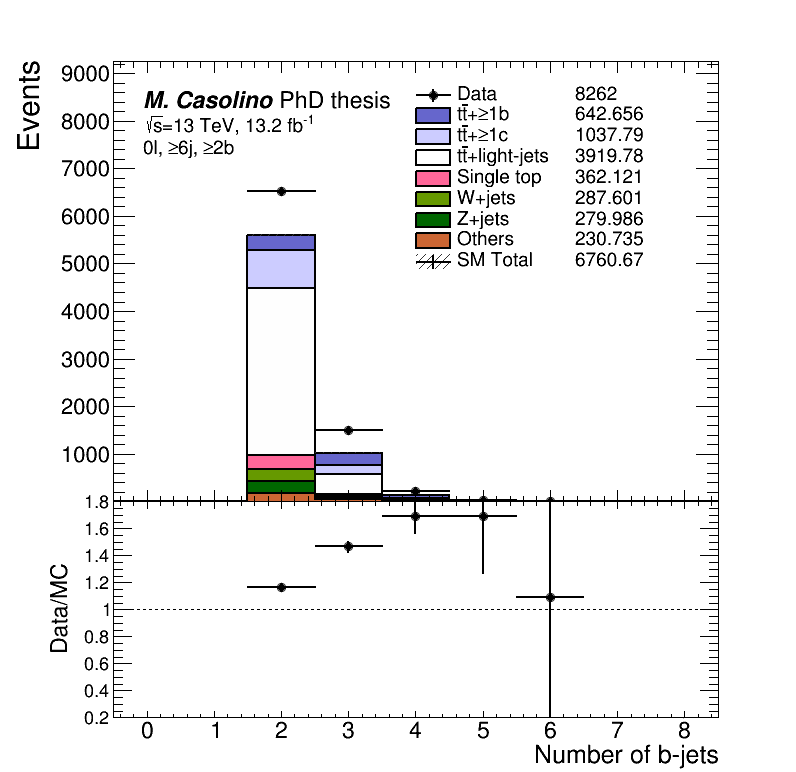
\includegraphics[width=0.9\textwidth]{figures/VLQ/presel/0lep/canv_c0l2b_bjets_n.png}
  \caption{}
  \label{}
\end{subfigure}
\begin{subfigure}{0.33\textwidth}
  \centering
  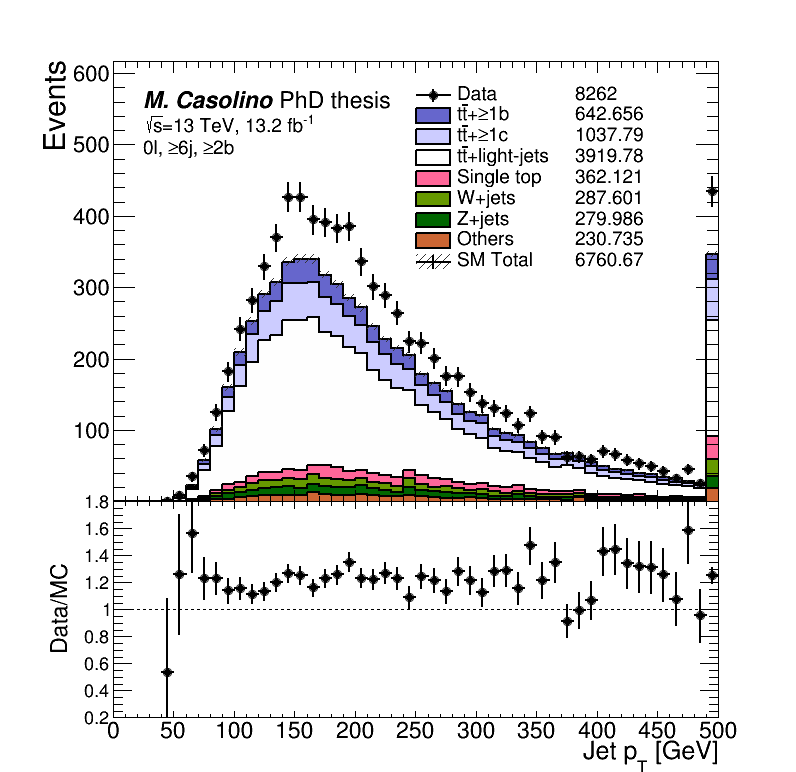
\includegraphics[width=0.9\textwidth]{figures/VLQ/presel/0lep/canv_c0l2b_jet0_pt.png}
  \caption{}
  \label{}
\end{subfigure}
\begin{subfigure}{0.33\textwidth}
  \centering
  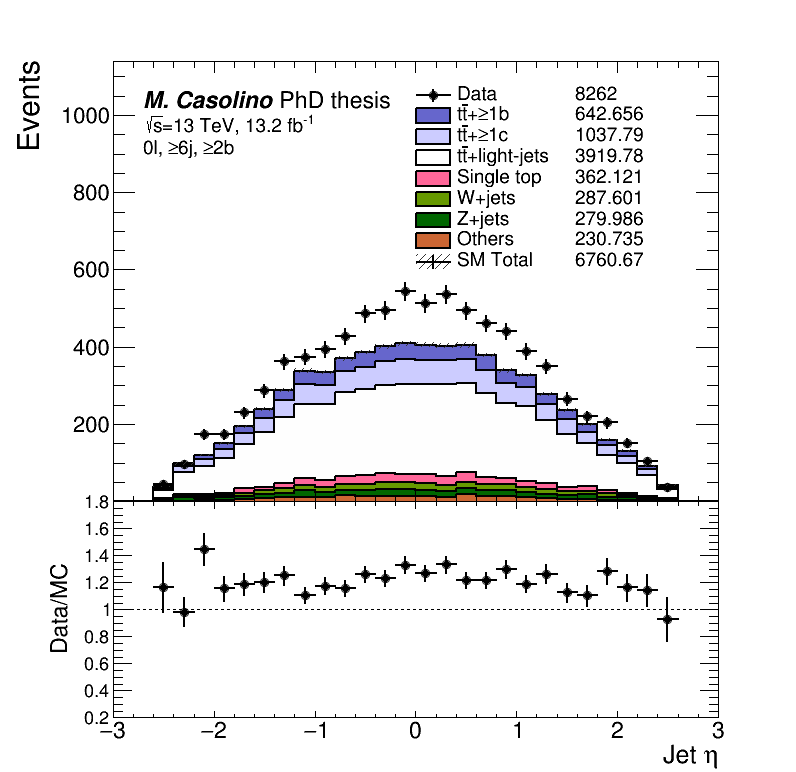
\includegraphics[width=0.9\textwidth]{figures/VLQ/presel/0lep/canv_c0l2b_jet0_eta.png}
  \caption{}
  \label{}
\end{subfigure}
\begin{subfigure}{0.33\textwidth}
  \centering
  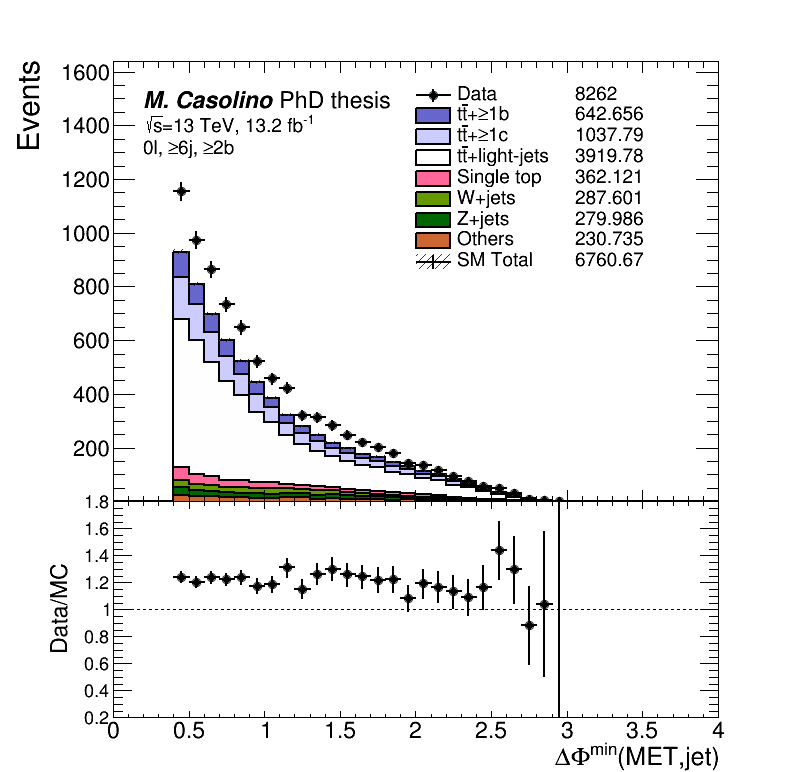
\includegraphics[width=0.9\textwidth]{figures/VLQ/presel/0lep/canv_c0l2b_dPhi_jetmet.png}
  \caption{}
  \label{}
\end{subfigure}
\begin{subfigure}{0.33\textwidth}
  \centering
  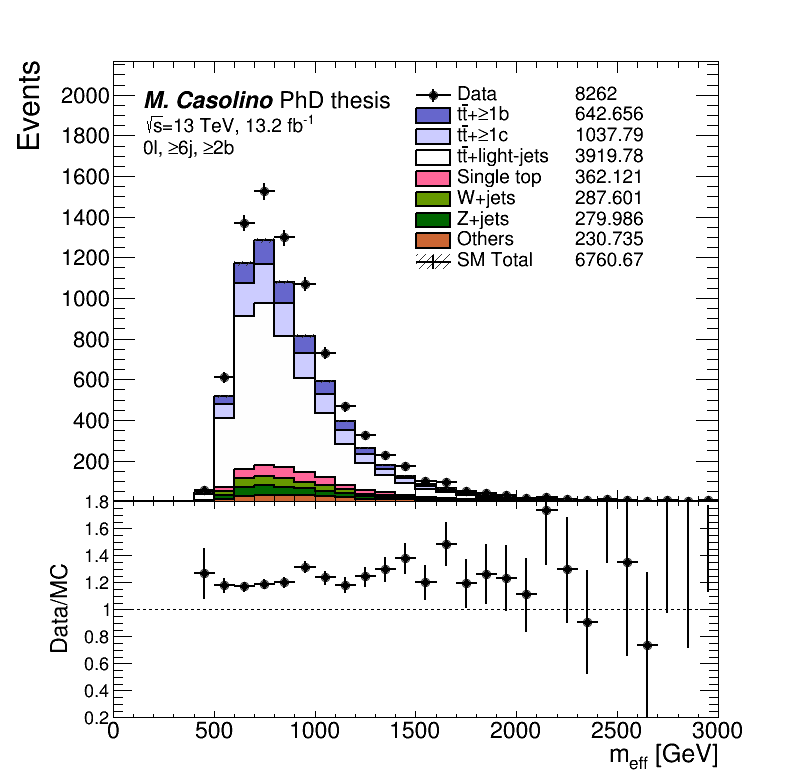
\includegraphics[width=0.9\textwidth]{figures/VLQ/presel/0lep/canv_c0l2b_meff.png}
  \caption{}
  \label{}
\end{subfigure}
\begin{subfigure}{0.33\textwidth}
  \centering
  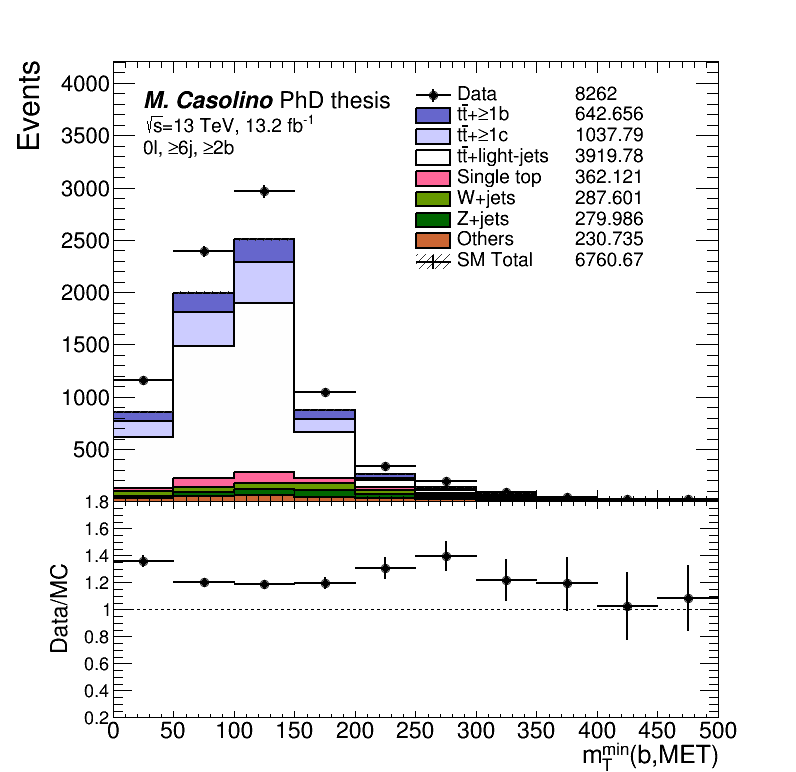
\includegraphics[width=0.9\textwidth]{figures/VLQ/presel/0lep/canv_c0l2b_mtbmin.png}
  \caption{}
  \label{}
\end{subfigure}
\begin{subfigure}{0.33\textwidth}
  \centering
  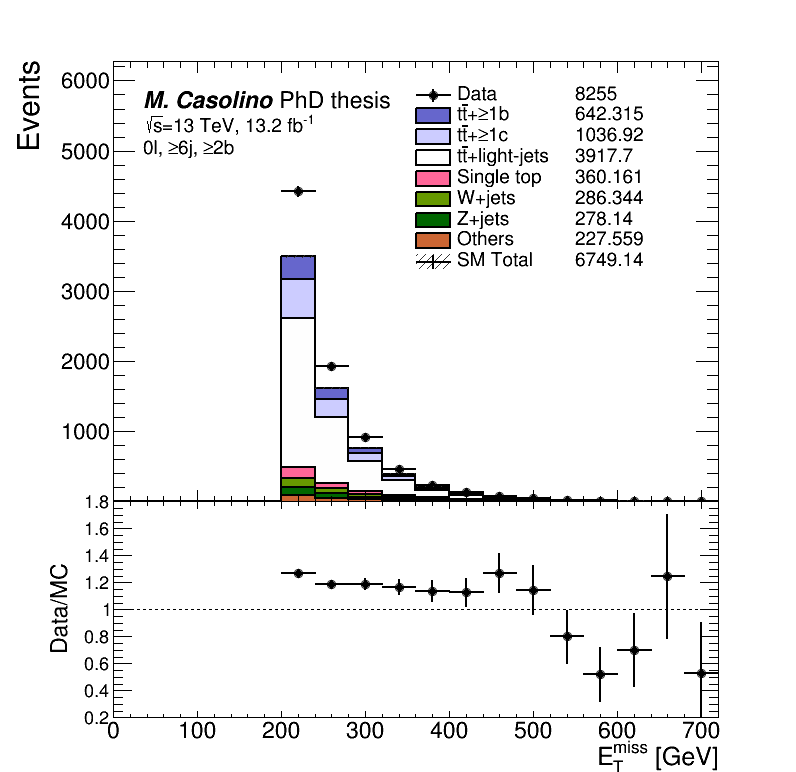
\includegraphics[width=0.9\textwidth]{figures/VLQ/presel/0lep/canv_c0l2b_met.png}
  \caption{}
  \label{}
\end{subfigure}
\begin{subfigure}{0.33\textwidth}
  \centering
  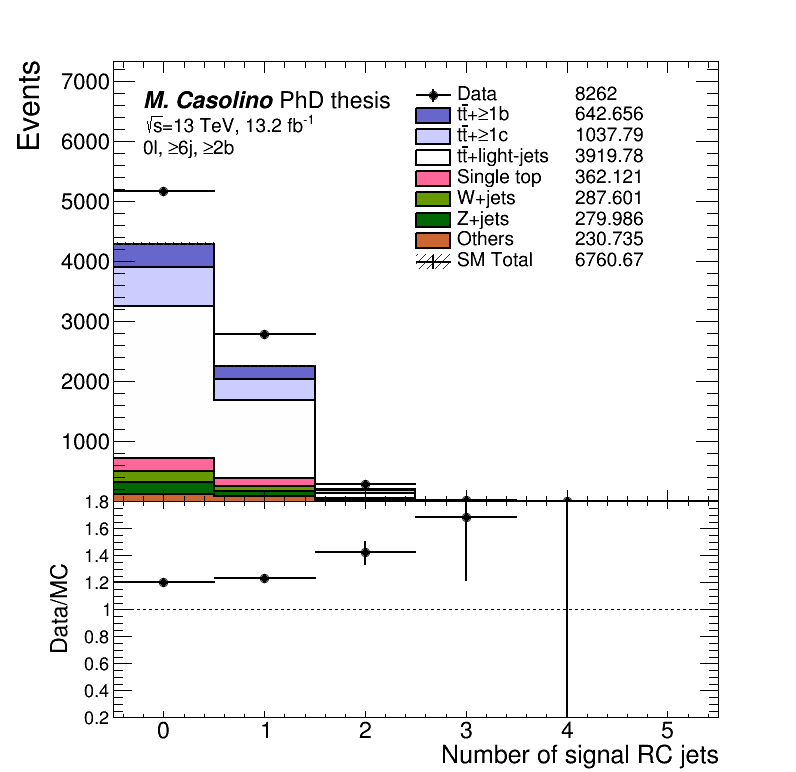
\includegraphics[width=0.9\textwidth]{figures/VLQ/presel/0lep/canv_c0l2b_RCjets_n.png}
  \caption{}
  \label{}
\end{subfigure}
\captionsetup{width=0.85\textwidth} \caption{\small Comparison between data and prediction in 0-lepton channel for (a) jet multiplicity, (b) $b$-tag multiplicity, (c) leading jet $\pt$ and (d) leading jet $\eta$, (e) $\Delta \phi_{\rm min}^{4j}$ , (f) $m_{\rm eff}$, (g) minimum transverse mass of the leading four $b$-jets and \MET ($m_{T,{\rm min}}^{b}$) , (h) \MET and (j) RT-jet multiplicity.}
\label{sec:vlq:fig:0ldatamc}
\end{figure}

Most of the observed discrepancies are covered by systematic uncertainties, which at the preselection level are
$\sim25\%$, dominated by jet energy scale, JVT SFs and $b$-tagging SFs. Additional contributions from the $\ttbar$ cross section and modelling cover the discrepancy in the jet multiplicity (see figure \ref{sec:vlq:fig:njetsyst}). A significant mismodelling in the $b$-jet multiplicity related to an underestimate of the $\ttbar+\ge1b$ cross section in {\sc Powheg+Pythia}, is not covered by systematic uncertainties since no uncertainty is assigned to it (see figure \ref{sec:vlq:fig:nbjetsyst}) as this background will be directly fitted from data. The treatment of systematics uncertainties is described in section \ref{chp:vlq:sec:syst}.

\begin{figure}[h!]
\begin{subfigure}{0.5\textwidth}
  \centering
  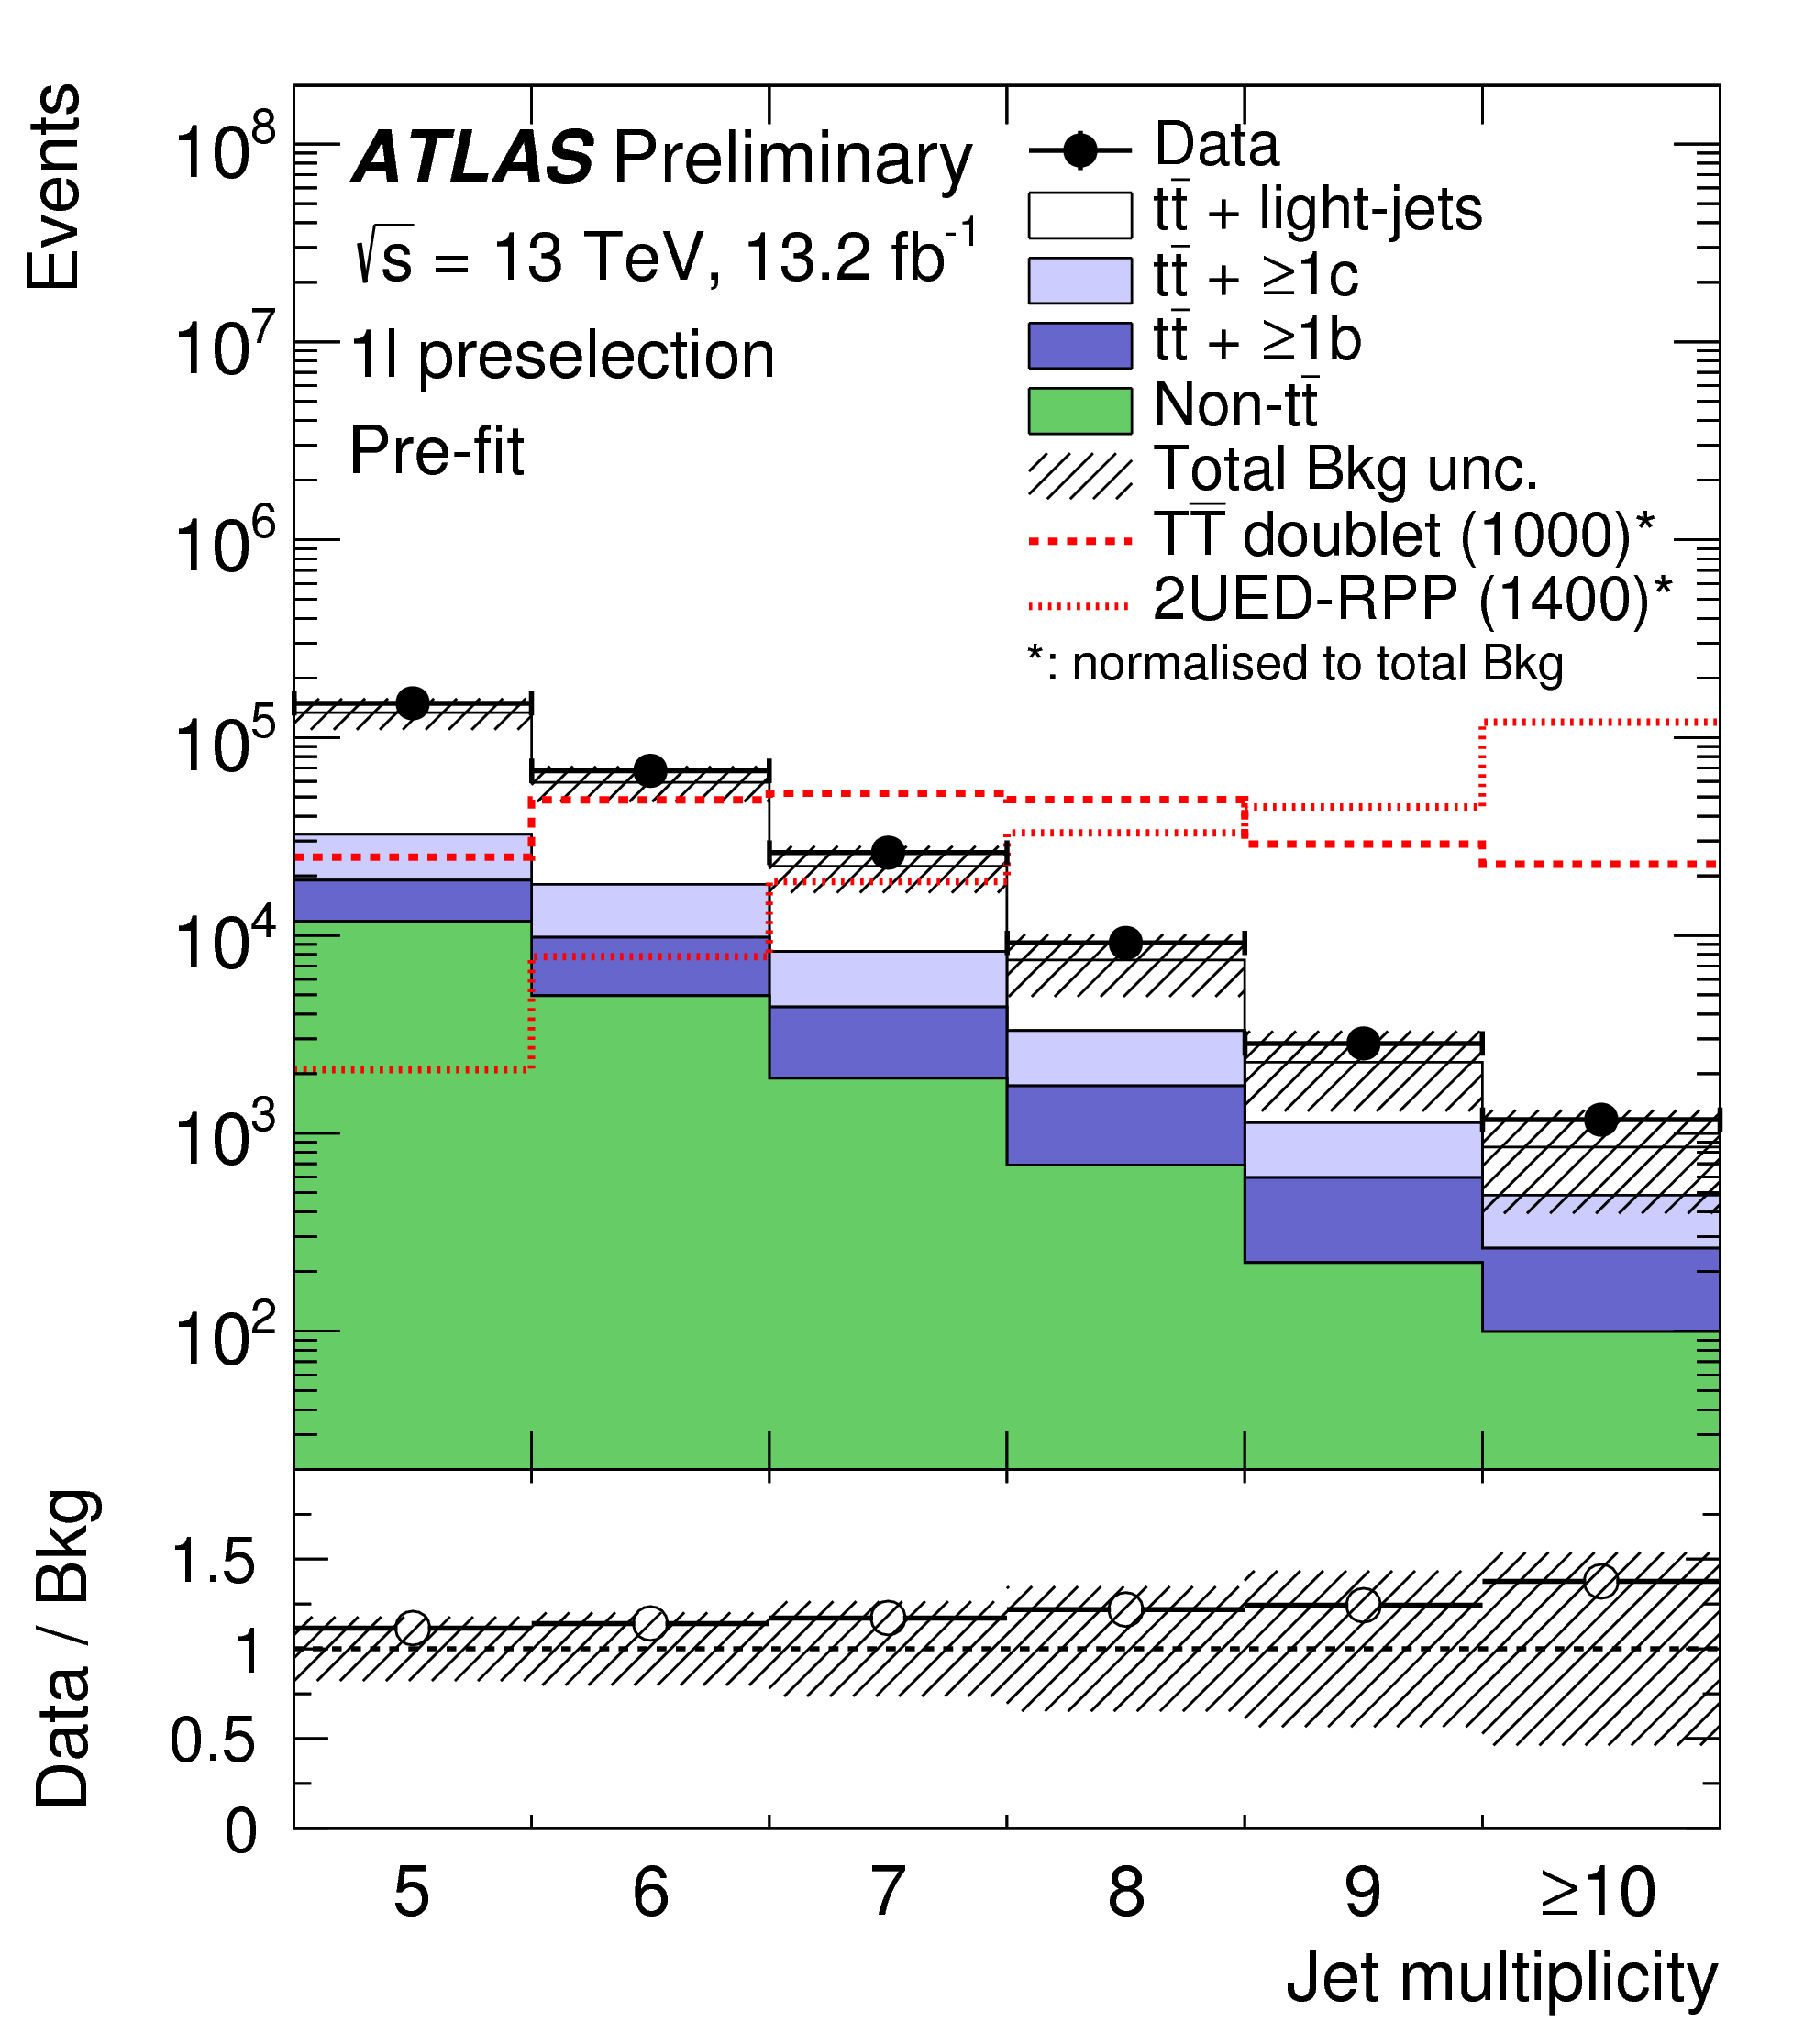
\includegraphics[width=0.9\textwidth]{figures/VLQ/figaux_01a.png}
  \caption{}
  \label{sec:vlq:fig:njetsyst}
\end{subfigure}
\begin{subfigure}{0.5\textwidth}
  \centering
  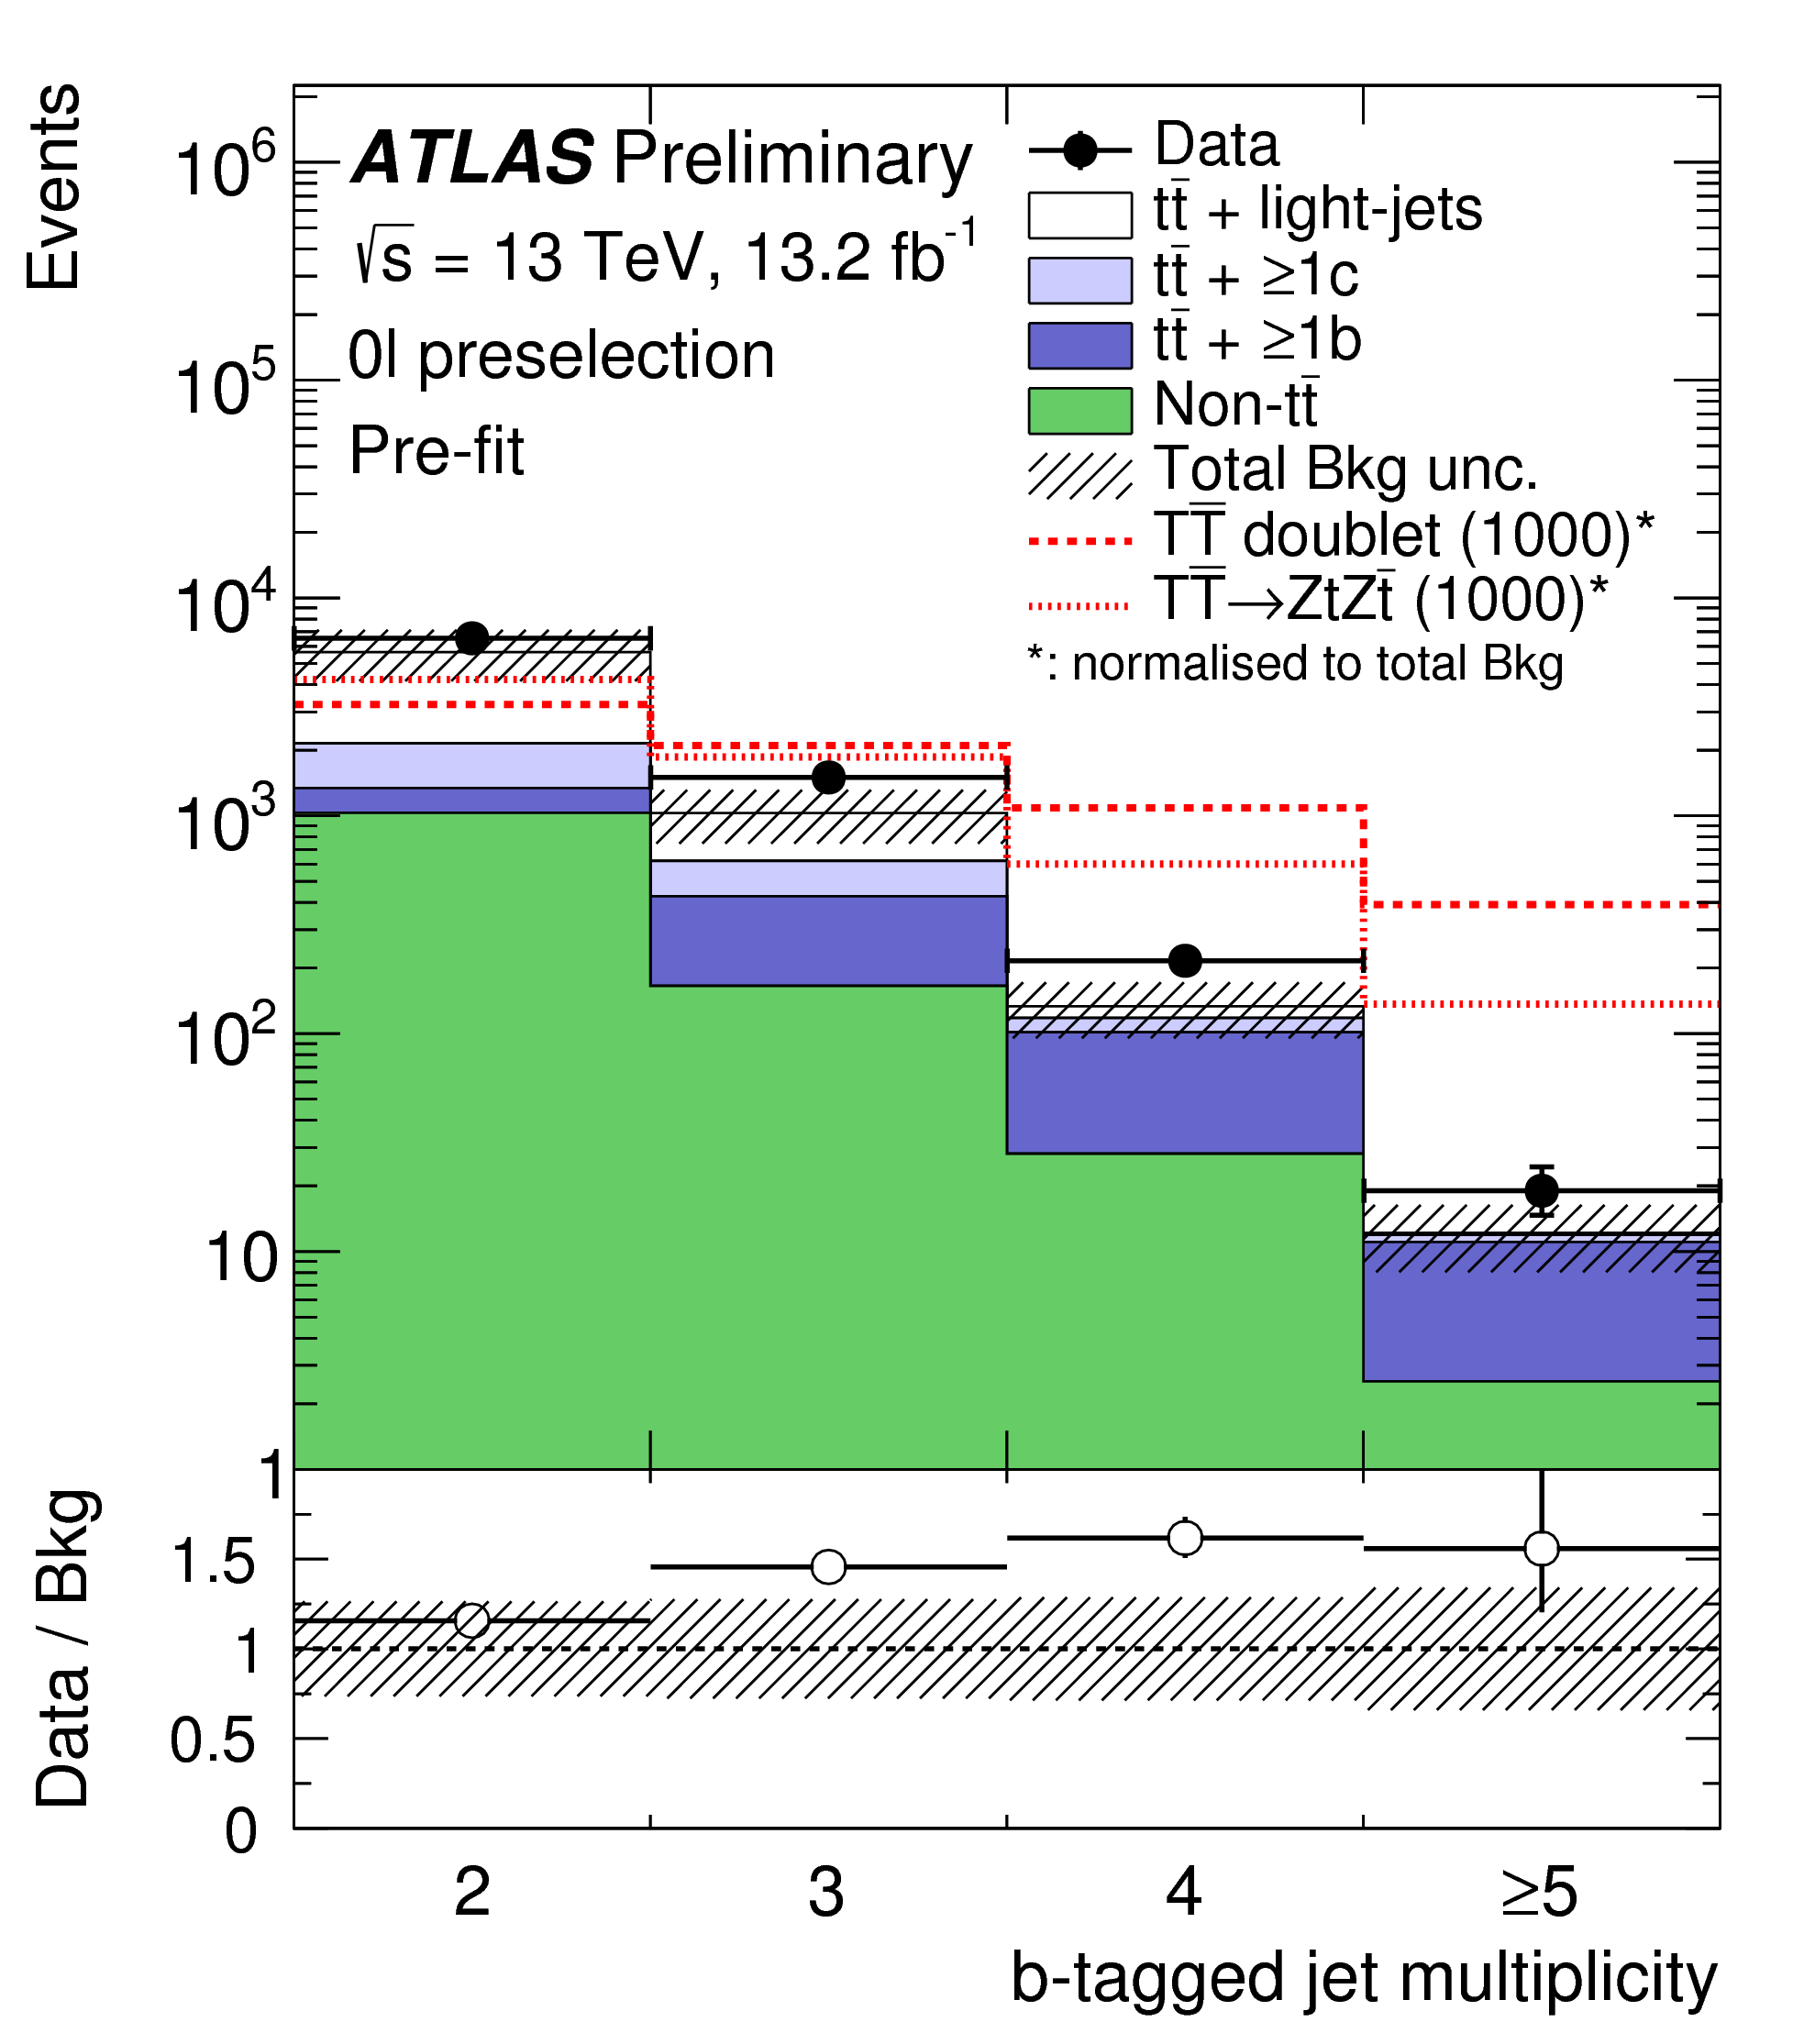
\includegraphics[width=0.9\textwidth]{figures/VLQ/figaux_02a.png}
  \caption{}
  \label{sec:vlq:fig:nbjetsyst}
\end{subfigure}

\captionsetup{width=0.85\textwidth} \caption{\small Comparison between data and prediction before performing the fit to data for (a) the jet multiplicity in 1-lepton channel and (b) the $b$-tag multiplicity in 0-lepton channel. The small contributions from $t\bar{t}V$, $t\bar{t}H$, single top, $W/Z$+jets, diboson, and multijet backgrounds are combined into a single background source referred to as ``Non-$t\bar{t}$''. The expected signal distributions are shown, normalised to the total background prediction, for three scenarios considered in this search: $T\bar{T}$ production in the weak-isospin doublet scenario and for ${\rm BR}(T\to Zt) = 1$ assuming $m_{T}$=1000 $\gev$ (red dashed and continuous histogram respectively), and $\ttbar\ttbar$ production within the 2UED/RPP model assuming $m_{KK}$=1400 $\gev$ (red dotted histogram). The last bin in all figures contains the overflow. The normalisation uncertainty on the $t\bar{t}+\ge1b$ background is not included in the background uncertainty band.}
\label{sec:vlq:fig:njetsnbjetsyst}
\end{figure}


%\begin{figure}[h!]
%\begin{subfigure}{0.5\textwidth}
 % \centering
  %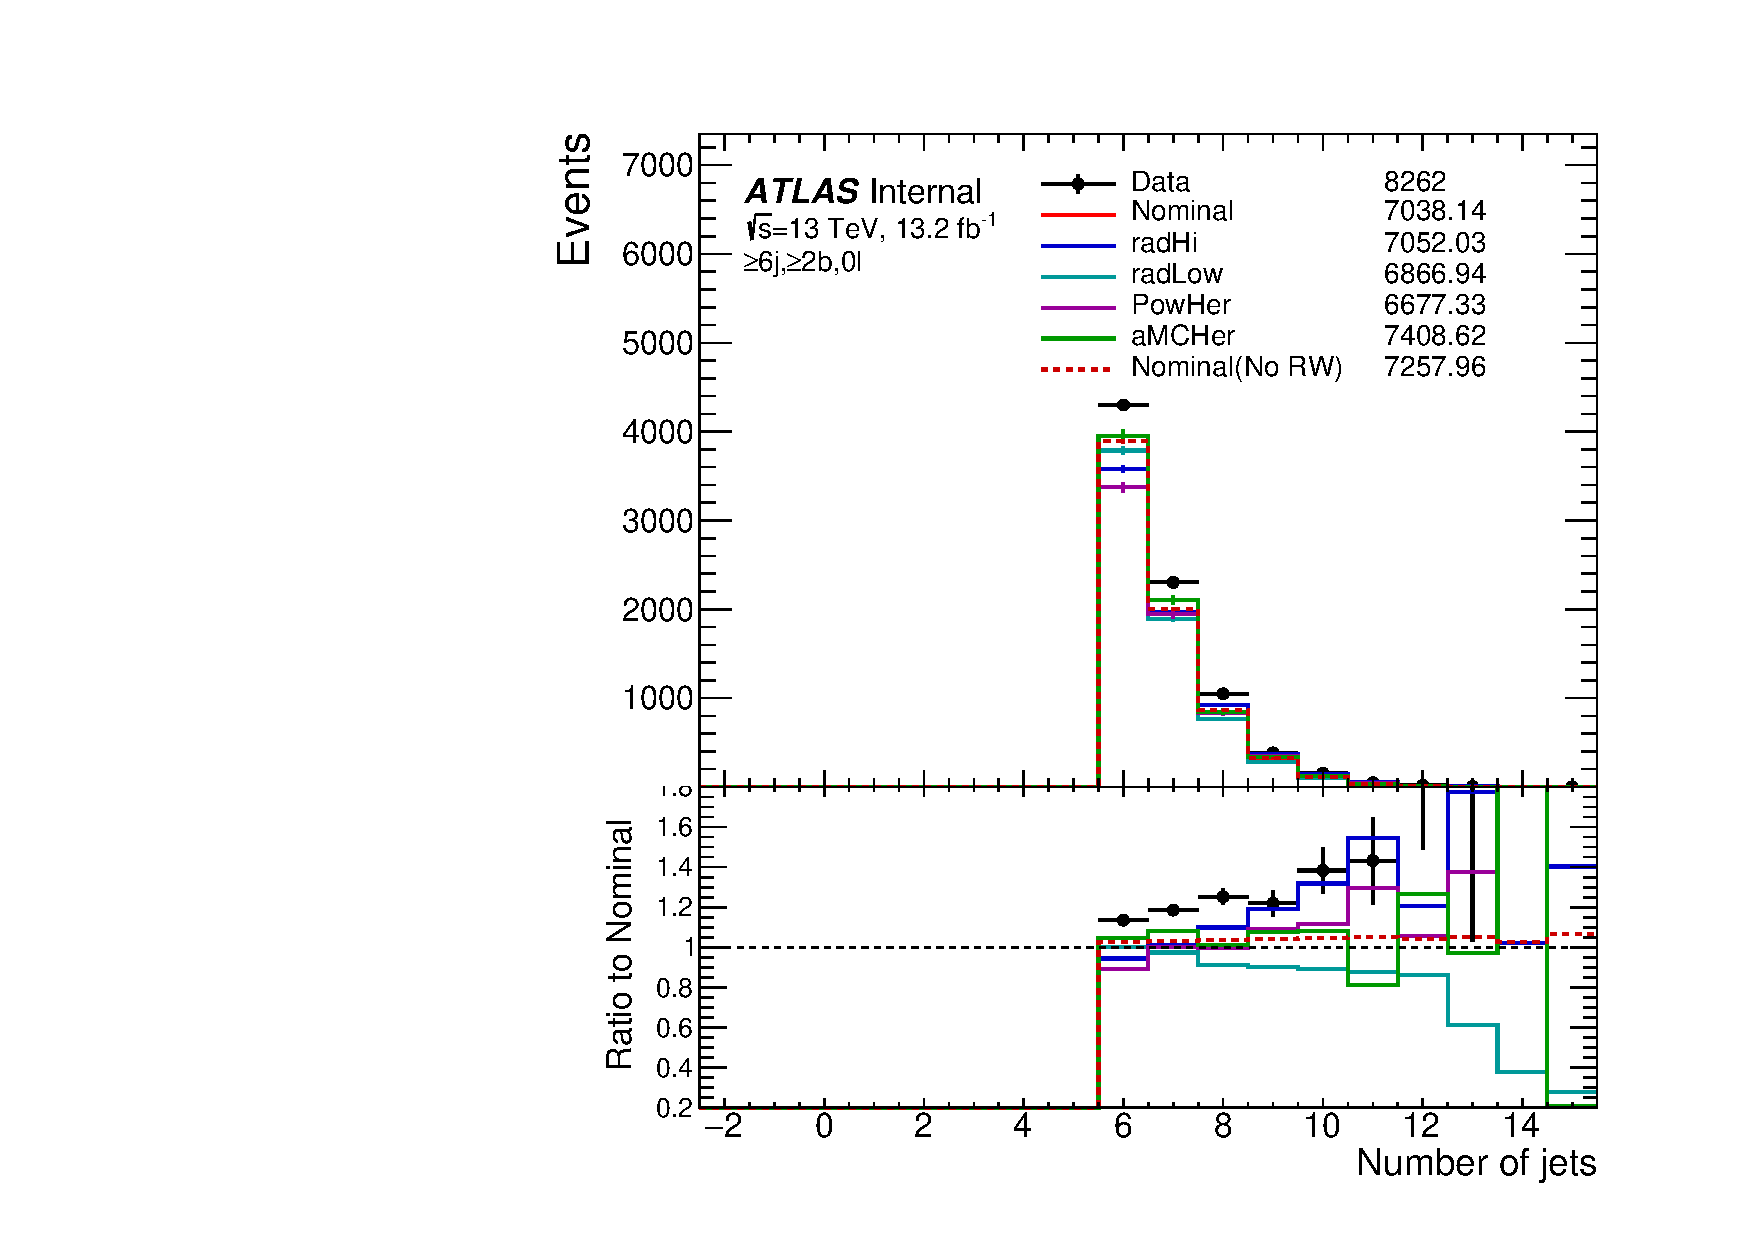
\includegraphics[width=0.9\textwidth]{figures/VLQ/canv_c0l2b_jets_n_ttbar.pdf}
  %\caption{}
  %\label{}
%\end{subfigure}
%\begin{subfigure}{0.5\textwidth}
 % \centering
 % 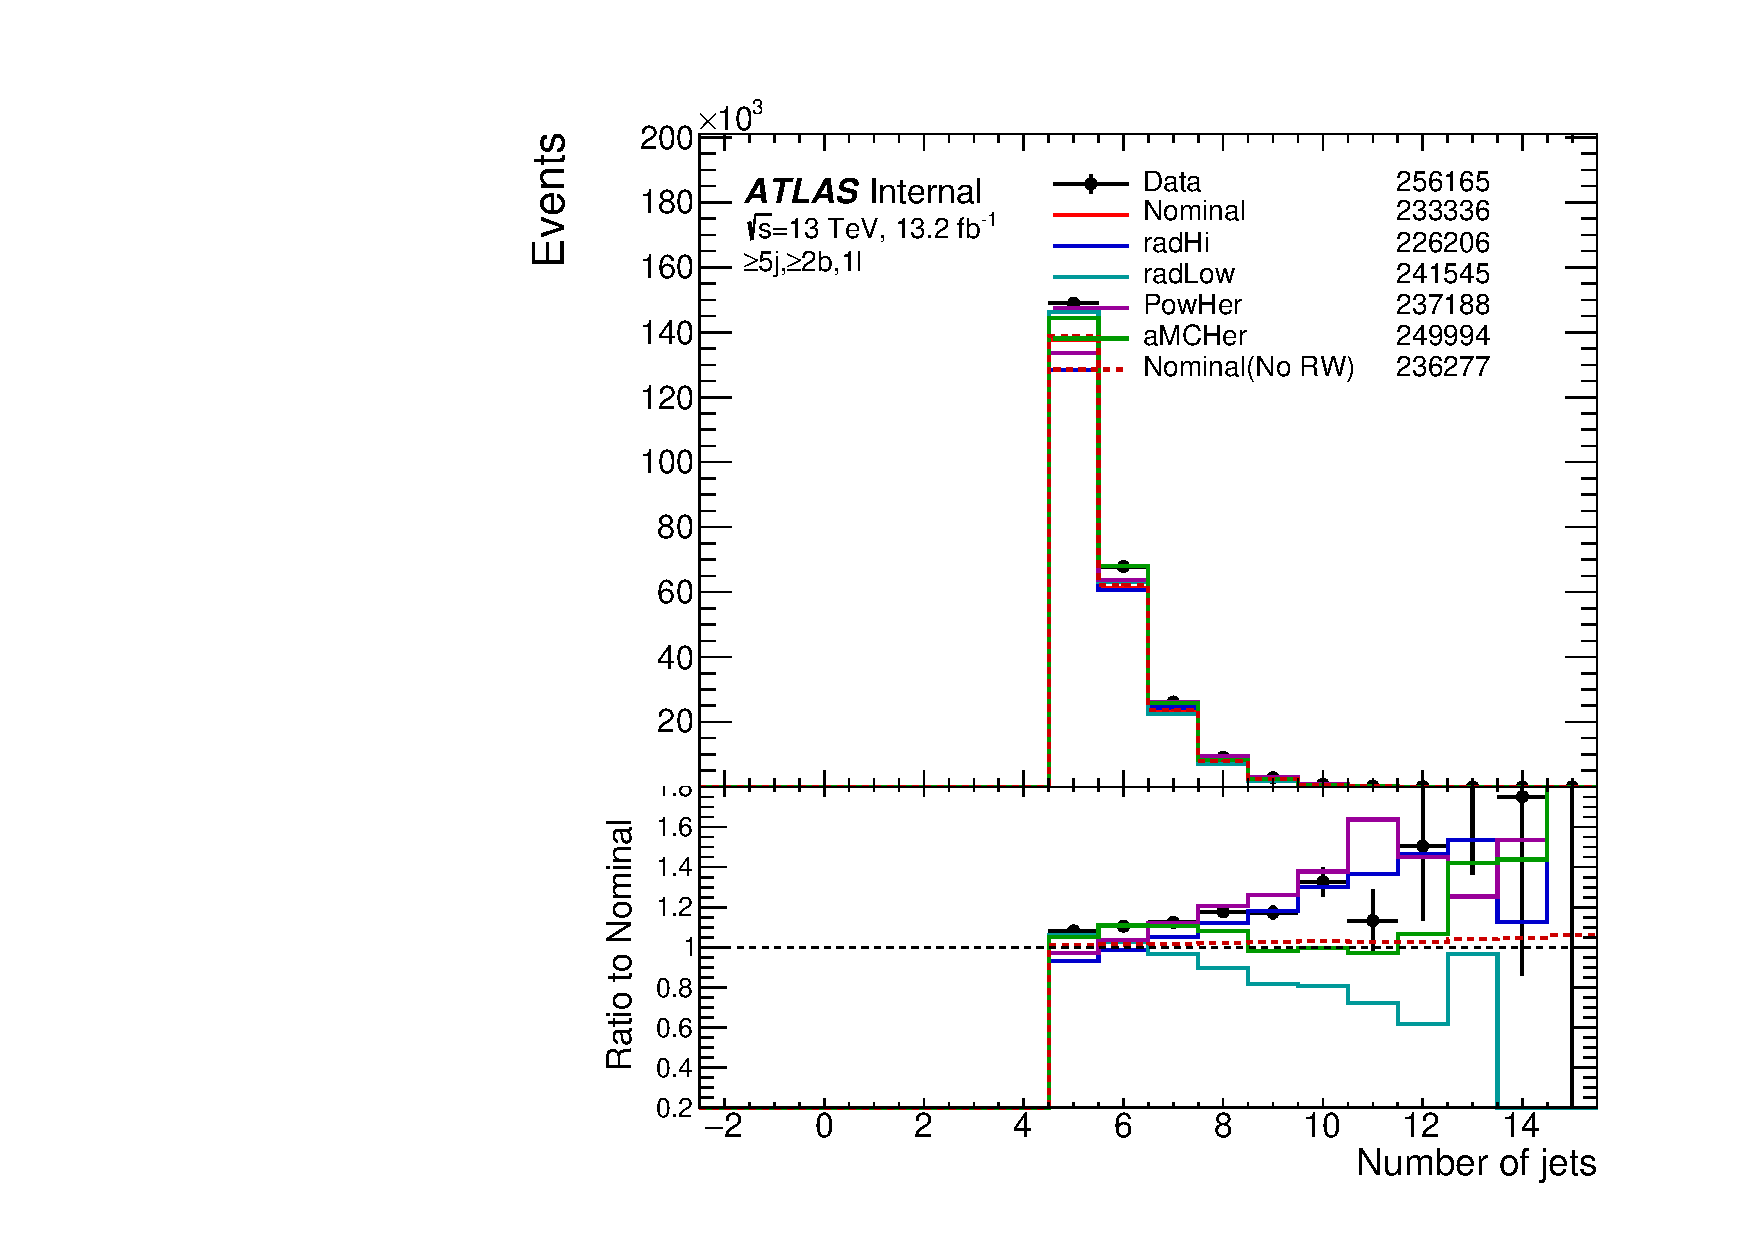
\includegraphics[width=0.9\textwidth]{figures/VLQ/canv_c1l2b_jets_n_ttbar.pdf}
  %\caption{}
  %\label{}
%\end{subfigure}

%\caption{Comparison between data and prediction in 0-lepton channel (a) and 1-lepton channel for jets multiplicity using different  $t\bar{t}+$jets generators.}
%\label{sec:vlq:fig:otherttbar}
%\end{figure}

